\documentclass[10pt]{article}
\usepackage{setspace}
\usepackage{amsmath,amssymb}
\usepackage{amsthm}
\usepackage{fancybox}
\usepackage{algorithm, algpseudocode}
\usepackage{url}

\usepackage{multirow}
\usepackage{color}
\usepackage{graphicx}
\usepackage{setspace}
\usepackage{comment}
\usepackage{bm}
\usepackage{enumitem}
\usepackage[breakable, theorems, skins]{tcolorbox}
\DeclareRobustCommand{\mybox}[2][gray!20]{%
\begin{tcolorbox}[   %% Adjust the following parameters at will.
        breakable,
        left=0pt,
        right=0pt,
        top=0pt,
        bottom=0pt,
        colback=#1,
        colframe=#1,
        width=\dimexpr\textwidth\relax, 
        enlarge left by=0mm,
        boxsep=5pt,
        arc=0pt,outer arc=0pt,
        ]
        #2
\end{tcolorbox}
}


\newcommand*{\KeepStyleUnderBrace}[1]{%f
  \mathop{%
    \mathchoice
    {\underbrace{\displaystyle#1}}%
    {\underbrace{\textstyle#1}}%
    {\underbrace{\scriptstyle#1}}%
    {\underbrace{\scriptscriptstyle#1}}%
  }\limits
}


\usepackage[margin=1in]{geometry}
 
\allowdisplaybreaks[4]
\usepackage{bbm}


\usepackage{amsrefs}
\usepackage{mathtools}
\mathtoolsset{showonlyrefs=true}


\usepackage[utf8]{inputenc}
\usepackage{hyperref}
\hypersetup{
    colorlinks=true,
    citecolor = blue,
    linkcolor=blue,
    filecolor=magenta,           
    urlcolor=black,
}

\usepackage[breakable, theorems, skins]{tcolorbox}
\DeclareRobustCommand{\mybox}[2][gray!20]{%
\begin{tcolorbox}[   %% Adjust the following parameters at will.
        breakable,
        left=0pt,
        right=0pt,
        top=0pt,
        bottom=0pt,
        colback=#1,
        colframe=#1,
        width=\dimexpr\textwidth\relax, 
        enlarge left by=0mm,
        boxsep=5pt,
        arc=0pt,outer arc=0pt,
        ]
        #2
\end{tcolorbox}
}

\def\sign{\textup{sgn}}
\theoremstyle{definition}
\newtheorem{thm}{Theorem}[section]
\newtheorem{lem}{Lemma}
\newtheorem{prop}{Proposition}
\newtheorem{pro}{Property}
\newtheorem{cor}{Corollary}[section]

\theoremstyle{definition}
\newtheorem{assumption}{Assumption}
\newtheorem{defn}{Definition}
\newtheorem{example}{Example}
\newtheorem{rmk}{Remark}
\usepackage{dsfont}

\theoremstyle{definition}
\newtheorem{open}[]{Open problems}

 \usepackage[parfill]{parskip}

\usepackage[compact]{titlesec}

\usepackage{sectsty}
\sectionfont{\fontsize{11}{10}\selectfont}
\subsectionfont{\fontsize{10.5}{10}\selectfont}
\usepackage[compact]{titlesec}
\titlespacing{\section}{0pt}{*0}{*0}
\titlespacing{\subsection}{0pt}{*0}{*0}
\titlespacing{\subsubsection}{0pt}{*0}{*0}

\input macros.tex

\begin{document}
\begin{center}
{\bf \large Beyond Matrices: Multi-task Learning Using Higher-order Tensors}\\
\vspace{.3cm}
\end{center}

\section{general theory of permutation equivalence models for tensors}

\subsection{Smooth}


\subsection{Isotonic}



My research is in the intersection of statistics, machine learning, and optimization, with a focus on tensor data analysis.
The proposed project is to develop a framework of statistical theory, machine learning methods, and efficient algorithms to analyze high-dimensional multiway array data. Recent advance in high-throughput sequencing technology has fundamentally transformed scientific research into a data-intensive filed. Through developing efficient methods for analyzing ``big data'', I strive to push the boundary of data science research further, in a form that is useful to individuals, academia, industry, and society. 

I have a unique combination of training backgrounds in mathematics (2006-2010), statistics (2010-2015), genetics (2015-2018), and computer science (2015-2018). I use mathematical language in my work, and math steers my creation to understand the fundamentals of the problems. On the other hand, I feel mostly fulfilled when the developed tools help scientists to make discoveries in the domain field. During my career, I am fortunately to have worked closely with many fellow scientists on cutting-edge big data problems, which have spurred new goals in my research and shaped my scientific approach. {\bf The prevailing theme in my research is to develop machine learning theory and methods to address multi-task, higher-order data challenges.} In this regard, my work will link machine learning and biomedical science, the two areas I have been working on extensively, and also develop new machine learning areas based on the questions raised in the applied endeavors.

\section{Research Goals and Significance}

\emph{Big data} has been a popular term one encounters everywhere, and we are told that data will define a new science. Rapid developments in modern technologies have made large-scale data readily available across science and engineering. Tensors, or multi-way arrays, provide a generalized data structure and serve as a foundation in many learning procedures. Methods built on tensors provide powerful tools to capture complex structures that lower-order methods fail to exploit. However, tensor-based methods are fraught with challenges. Extending familiar matrix concepts to tensors is notably difficult, and most computational problems regarding tensors are NP-hard. Analyzing tensor data with increasing dimensionality and growing complexity presents serious challenges --- the classical off-the-shelf methods cannot keep up with them, and new approaches have to be developed. 

Below I give two examples of biomedical tensor data arising from my current collaborations, and I will propose new linkages between tensor data analysis with machine learning research. 

{\bf Multi-tissue, multi-individual gene expression.} A typical multi-tissue experiment collects gene expression profiles from different individuals in a number of tissues. The recent completion of Genotype-Tissue Expression (GTEx, Figure 1a) project has provided unprecedented opportunities to investigate transcriptome diversity and complexity. The study results in a huge compendium of tensor data consisting of millions of expression measurements from $\sim$ 20,000 genes across 544 individuals and 53 human tissues, including 13 brain regions, adipose, heart, artery, skin, and more. In this setting, variation in the expression levels arises due to contributions specific to genes, tissues, individuals, and interactions thereof. Understanding the multifactorial patterns of whole-genome transcriptome variation is crucial to unravel gene networks and tissue functions, thereby broadly facilitating research efforts to unravel genetic basis for personalized disease.

{\bf Multimodal neuroimaging data analysis.} Neuroimaging data analysis aims to characterize the human brain connectivity in response to stimulus or physiological changes. As of the fall of 2020, the human connectome project (HCP) has released massive datasets representing the anatomical and functional connectivities within human brains from over 1,200 individuals. Adjacency matrices (networks) are common tools to describe the brain connectivity, where edges (connections) join a set of nodes (brain voxels). Different imaging measurements are utilized to construct the brain networks (Figure 1b), including functional magnetic resonance imaging (fMRI), electroencephalography (EEG), and diffusion tensor imaging (DTI). A key feature is that the acquired networks are huge in size and each possesses complex spatial temporal structure. Efficient methods for multi-modal learning are essential for investigating the commonality and variability between the networks. 

\begin{figure}[H]
\begin{center}
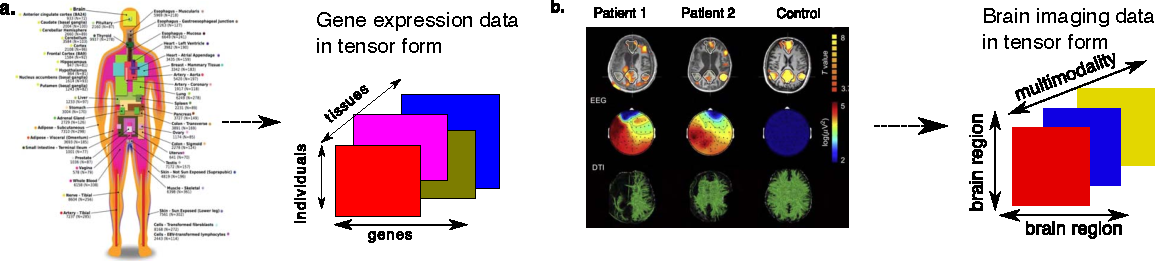
\includegraphics[width=1\textwidth]{example.pdf}
\caption{\small (a) GTEx project collects gene expression profiles of over 20,000 genes from 544 individuals across 53 human tissues. Figure modified based on Timpson et al. [2018]. (b) HCP collects multimodal imaging data including EEG, DTI, fMRI from over 1,200 individuals. Figure modified based on Bruno et al. [2011].}
\end{center}
\end{figure} 

In the above two examples and many others applications, scientists are interested in identifying interpretable low-dimensional structure within the high-dimensional tensor data. The research question goes beyond the traditional multivariate analysis: we are interested in the distribution over network-valued ``objects'' where the objects can be images, networks, manifolds, and arrays. {\bf The main approach in my research is to develop a framework of machine learning models, scalable algorithms, and user-friendly software to analyze multi-modal tensor data.} This will allow practitioners to examine complex interactions among tensor entries and between multiple tensors, thereby providing solutions to questions that cannot be addressed by traditional analysis.  

My general strategy is to carve out a broad range of specially-structured tensors that are useful in practice, and to develop efficient machine learning methods for analyzing these high-dimensional tensor data. Accordingly, the proposed projects will provide a machine learning framework in three aspects to facilitate high-dimensional tensor data analysis. The PI’s previous research on bridging tensors to matrices~\cite{wang2017operator,zeng2019multiway,wang2018learning,wang2017tensor,wang2019three,lee2020tensor} has led to a new inquiry on machine learning techniques for tensors. The proposed research is built upon the PI's past breakthrough but also opens up a suite of theory, methodology, and practice for analyzing high-dimensional tensor data in applications. 

{\bf Aim 1: Spectral theory for specially-structured tensors.} Tensors are not simply matrices with more indices; rather, they are objects possessing multilinear algebraic properties. The proposed research will focus on several spectral quantities for deterministic tensors and random tensors. The techniques developed will facilitate the development of novel tensor-based modeling and computations. See Section~\ref{sec:aim1}.

{\bf Aim 2: Unsupervised learning with high-dimensional tensors.} Many real-world multiway datasets are instances of high-dimendional tensors, in which tensor entries take on discrete values (e.g., ranking) or binary indicators 0/1 (e.g., presence vs.\ absence). Discrete measurements are notably harder to analyze because of the limited information. The proposed research will (1) show how current estimators are suboptimal, (2) develop new estimators that obtain faster rates of convergence, and (3) enrich the application domains in signal processing and network analysis. See Section~\ref{sec:aim2}.

{\bf Aim 3: Supervised Tensor Decomposition with Interactive Side Information.} Machine learning prediction problems common arise in daily applications, i.e.,\ identifying segmentations from images, classifying documents into topics, or deciding target customers in recommendation systems. These problems are often formulated as predicting a variable $Y$ from explanatory variables $X$, where the sample available is in the form of pairs $\{(X_i, Y_i): i=1,\ldots,n\}$. In contrast to traditional work that focuses on only univariate response, we will develop a general learning framework with tensor observation as a response, and features on multiple modes as predictors. Incorporating multiple side information greatly improves the prediction accuracy in tensor data. See section~\ref{sec:aim3}.

{\bf Research team and PI's qualification}. The PI is a young female faculty in the Department of Statistics at UW-Madison. The PI is also a core member in the Institute for Foundations of Data Science (IFDS) which is a joint initiative between Computer Science, Statistics, Mathematics and Electronical Engineering. The proposed research is built upon the PI’s established methodological work on functional properties of higher-order tensors~\cite{wang2017operator, wang2017tensor,zeng2019multiway,wang2018learning,lee2020tensor} and applied work on tensor-based genomic research~\cite{wang2019three,wang2018two}. The PI’s previous work has a transformational nature involving connections across diverse disciplines, and the PI strives to push the boundary of interdisciplinary research further.

To accomplish the proposed research goals, the PI plans to devote four months to each of the three projects. Estimation methods, machine learning algorithms, and computational performance will be carefully studied. Applications to data-intensive fields especially in recommendation system and personalized medicine will be emphasized. The funded PhD students and Postdoc will contribute to aims 1--3. Undergraduate students will also participate in various aspects of the research. These aims will be incorporated into research training and machine learning eduction of students. The PI’s group will also develop publicly available software packages that are ready for use by practitioners.


\section{Research Goals and Strategies} 
The proposed project focuses on tensors of order 3 or greater, known as higher-order tensors. A tensor $A \in  \mathbb{R}^{d_1 \times\cdots \times d_K}$ is a higher-order generalization of matrix, and $A$ can be viewed as a multilinear functional that maps $K$-tuples of vectors to numbers: $(x_1,\ldots,x_K)  \mapsto A(x_1,\ldots,x_K) \in \mathbb{R}$. However, higher-order tensors are not simply matrices with more indices; rather, they are data objects possessing special  properties. The computational challenge stems from the gap from linear algebra to multilinear algebra. The multilinearity is an active topic that is currently studied in complexity theory; tensor computation has been shown to closely connect to the long-standing problems in computer science: P vs.\ NP and matrix multiplication. 

Below I outline three main directions I plan to pursue with the Sony research grant. This would build new links between machine learning methodology and scientific discovery, and also produce new areas in which machine learning theory and applications combine and complement each other. 


\subsection{Computational Foundations for Specially-Structured Tensors} \label{sec:aim1}
This aim focuses on the spectral properties of higher-order tensors. Here I take the operator norm for illustration but other spectral properties can similarly be studied. The operator norm of a tensor is characterized by the best rank-one approximation in the least square sense. Given an order-$K$ tensor, each possible unfolding operation is represented using a partition $\pi$ of $\{1, . . . , K\}$, where a block in $\pi$ corresponds to the set of modes that are combined into a single mode. Figure 2 illustrates an example for $K = 3$. Earlier I have established a new framework representing all possible tensor unfoldings using the partition lattice, and I show that the spectral norm comparison bounds scale polynomially in the tensor dimensions $\{d_n\}$ with powers depending on the corresponding partition and block sizes. The operator norms of all possible tensor unfoldings together define what we coin a ``norm landscape'' on the partition lattice. To our knowledge, this is the first result to provide a full picture of the norm landscape over all possible tensor unfoldings.

\begin{figure}[http]
\centering
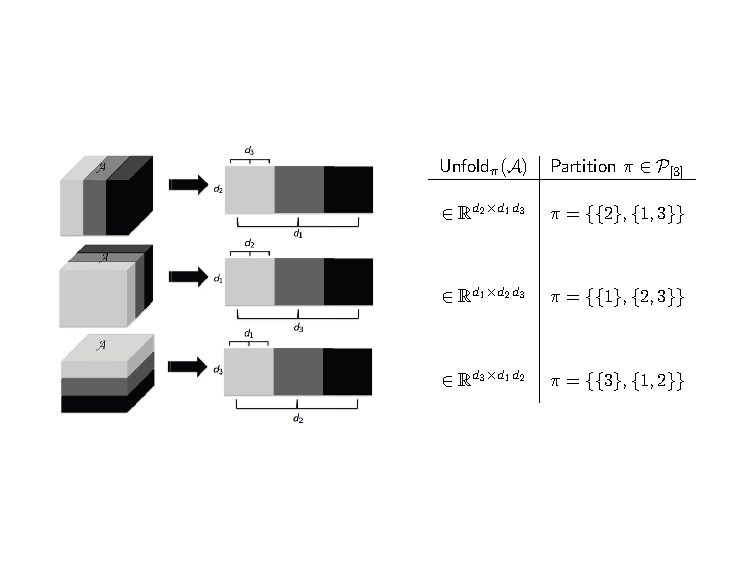
\includegraphics[width=.62\textwidth]{flattern.pdf}
\caption{\small An order-$3$ tensor and its matricizations. The set of all possible unfoldings is in one-to-one correspondence with the set of partitions of $\{1,2, 3\}$.
} \label{fig:1}
\end{figure}


My earlier results are already useful in several machine learning applications but should be interpreted with caution: the comparison bounds concerns the worst-case scenarios with arbitrary tensors. Tensors arisen in applications are often specially-structured. The structures of interest include, but are not limited to, low-rankness, sparsity, non-negativity, orthogonality, and block structure. We plan to study a range of spectral properties of these tensors. I expect that our newest attempt that focuses on structured tensors will provide the right framework to take this one step further. We will not only show the spectral properties of general tensors, but also finely disentangle the structured signals with the less-structured stochastic noise. These will provide machine learning foundations to novel tensor-based learning algorithms. 


\mybox[gray!20]{{\bf Breaking previous limits:} We plan to investigate the spectral properties for both deterministic and random tensors. For example, do the higher-order tensors require a completely new modeling paradigm compared to traditional matrix data? Solving these questions would nicely connects multilinear optimization to machine learning applications.}


\subsection{Unsupervised Learning with High-dimensional Tensor Data}\label{sec:aim2}
My goal in this direction is to develop unsupervised learning tools, i.e., clustering, denoising, and dimension reduction, for high-dimensional tensors, where the learner has little or no label information during training. This is an area where modeling and validation are notably difficult due to missing information. My group has recently developed an efficient tensor decomposition method to successfully estimate salient blocks in the multi-relational network data. Our clustering algorithm discovers community structure with higher accuracy, while being $11\times$ faster, than the competing methods~\cite{wang2019three,zeng2019multiway,wang2018learning}. We are currently generalizing the methods for integrative analysis of multimodal networks. The work will unlock several ambitious directions that lead to robust decision-making in science and engineering applications including electronic industry.  


\subsubsection{Interplay between Statistical Performance and Computational Efficiency}
Tensor decomposition problems arise frequently in applications such as neuroimaging, recommendation system, topic modeling, and sensor network localization. Developing efficient and accurate algorithms for tensor decomposition receives much attention recently. My goal is to develop efficient tensor methods with theoretical guarantees and to make use of the powerful tensor tools for elucidating complex structure in multi-mode data. In the simplest form, tensor decomposition can be formulated as finding the latent factors $\{\mathbf{u}_r\}$ from a noisy tensor $\hat \tA\in(\mathbb{R}^{d})^{\otimes K}$,
\begin{figure}[H]
\centering
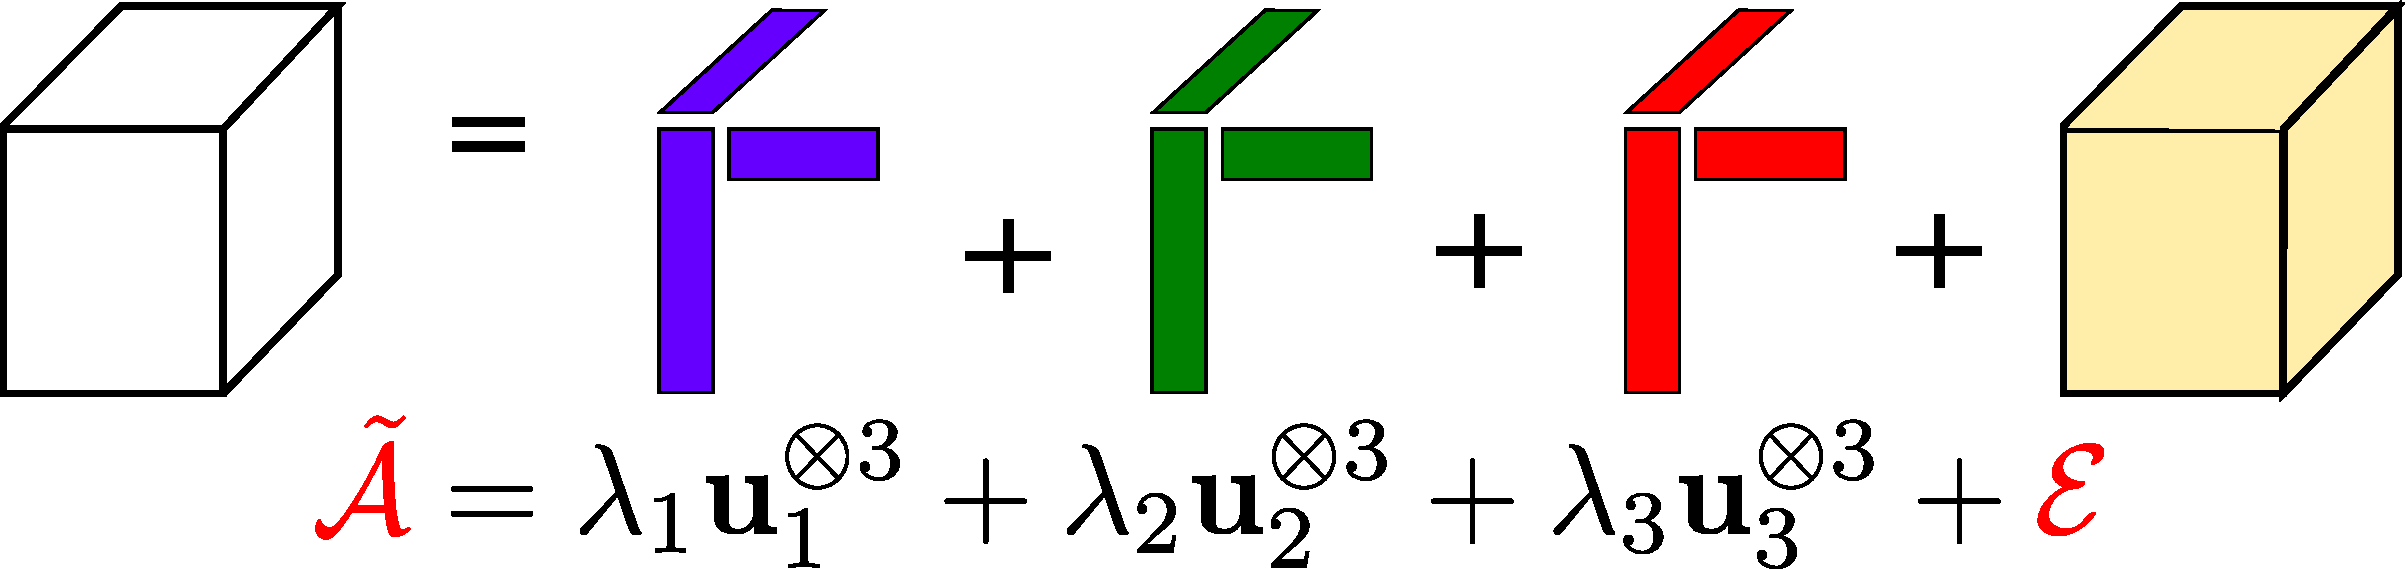
\includegraphics[width=.5\textwidth]{nearly_SOD2.pdf}
\caption{Schematic figure for unsupervised tensor decomposition}\label{fig:3}
\vspace{-.5cm}
\end{figure}
where the $\Theta:=\sum_{r=1}^R \lambda_r \mathbf{u}_r^{\otimes K}$ is called the signal tensor, $\{\mathbf{u}_r\}$ is a set of unit vectors in $\mathbb{R}^d$, $\lambda_i$s are positive scalars in $\mathbb{R}$, and the perturbation $\tE$ represents a small, stochastic noise tensor. 

Classical machine learning theory only studies the asymptotical estimation properties when the computational resource is unlimited. However, modern data science is more concerned on the trade-off between statistical limit and computational efficiency. In this regards, we aim to study the fundamental problems of structured tensor decomposition, including the signal-to-noise ratio under which a reliable algorithm is possible, the intrinsic hardness, in terms of minimax rate, of the estimation problem, the estimation properties that are specific to a particular algorithm, and those general to all algorithms. My preliminary results reveal that, for a broad range of low-rank tensors, the empirical estimate often exhibits a two-component error bound:
\[
\text{Loss}(\hat \Theta^{(t)}, \Theta_{\text{true}}) \leq \KeepStyleUnderBrace{C_1 \rho^t\text{Loss}(\hat \Theta^{(0)},\ \Theta_{\text{true}})}_{\text{algorithmic error}}+\KeepStyleUnderBrace{C_2 d^{-(K-1)/2}}_{\text{statistical error}},
\]
where $\hat \Theta^{(0)}$ is the initialization, $\hat \Theta^{(t)}$ is the estimation at the $t$-th iteration, $\rho\in(0,1)$ is a contradiction parameter, and $C_1,C_2>0$ are two constants that do not depend on dimensions. This bound reveals the interesting interplay between the computational and statistical errors, and the result immediate suggests a practical tradeoff between the two aspects. Understanding the gap between the algorithm property and statistical optimality is one of our main goals, which will in turn offer a useful guide to algorithm designs.


\subsubsection{Preliminary Applications to Human Connectome Project (HCP)} 
My group is currently applying the tensor decomposition methods to neuroimaging studies~\cite{geddes2016human}. We use the unsupervised tensor method to analyze an ordinal tensor consisting of structural connectivities among 68 brain regions for 136 individuals from Human Connectome Project (HCP). Each entry in the HCP dataset takes value on a nominal scale, \{{\it high, moderate, low}\}, indicating the strength level of fiber connection. We convert the dataset to a 3-level ordinal tensor $\tA\in[3]^{68\times 68\times 136}$, and apply the ordinal tensor method with a logistic link function. Based on the estimated tensor factors $\mathbf{\hat u}_r$, we perform a clustering analysis via K-mean on the brain nodes. The 68 brain nodes are grouped into 11 clusters. We find that the clustering captures the spatial separation between brain regions very well (Table~\ref{table:clustering}). In particular, cluster I represents the connection between the left and right hemispheres, whereas clusters II-III represent the connection within each of the half brains (Figure~\ref{figure:brain image}). Other smaller clusters represent local regions driving by similar nodes. For example, the cluster IV/VII consists of nodes in the supramarginal gyrus region in the left/right hemisphere. This region is known to be involved in visual word recognition and reading. The identified similarities among nodes without external annotations illustrate the potential power of tensor methods to clustering analysis. 


\begin{figure}[ht]
\centering
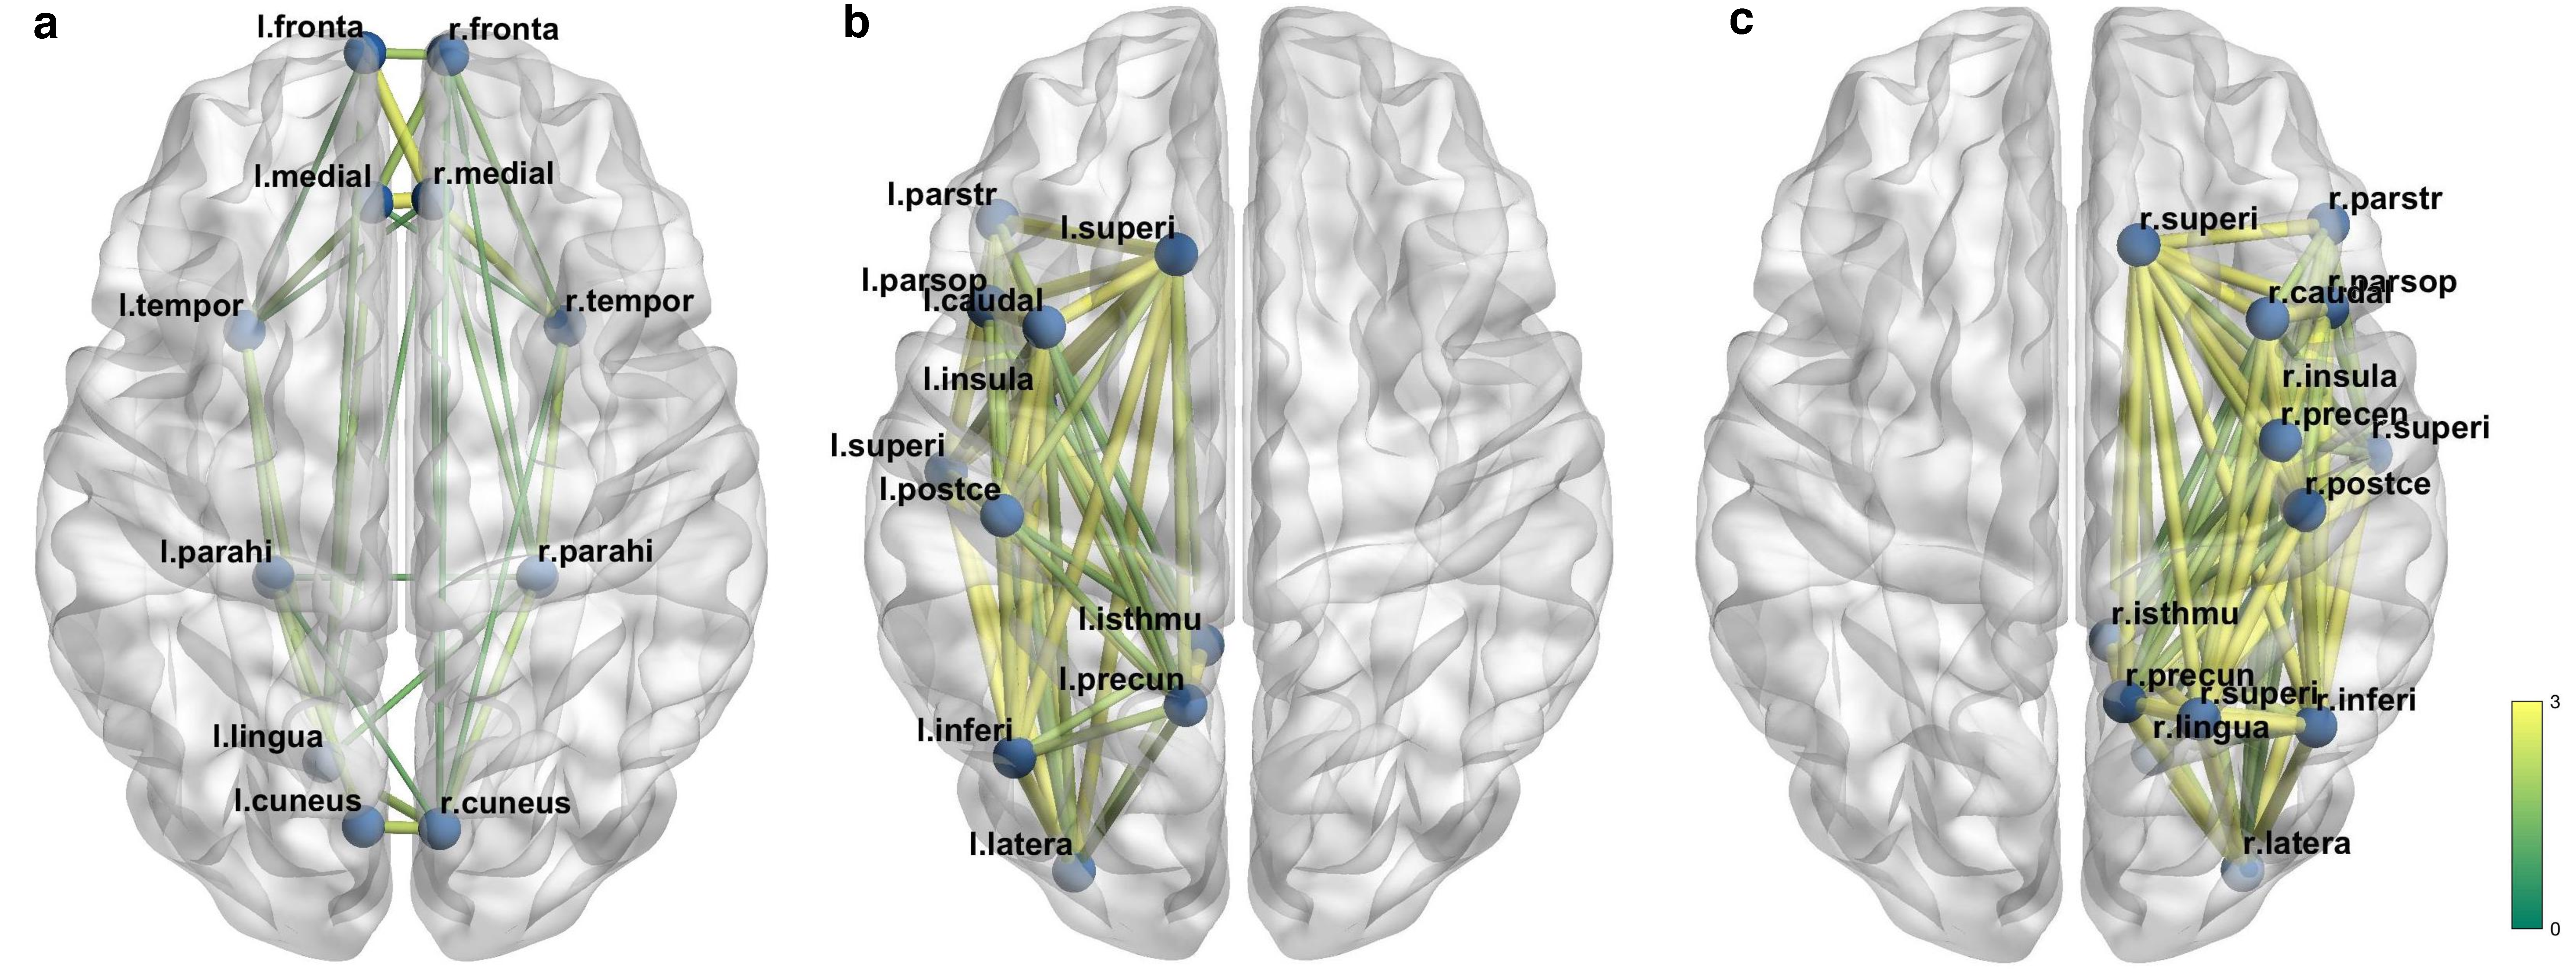
\includegraphics[width = .7\textwidth]{HCP.pdf}
\caption{Tensor clustering methods applied to neuroimaging data. Cluster I reflects the connections between two brain hemispheres (a). Cluster II/III consists of nodes within left/right hemisphere (b-c). Node names are shown in abbreviation. Edges are colored based on predicted connection level averaged across individuals. }  \label{figure:brain image}
\end{figure}


\begin{table}[ht]
\center
\begin{sc}
\resizebox{\columnwidth}{!}{
\begin{tabular}{|c|c|c|c|}
\hline
Cluster     & \multicolumn{3}{c|}{I}\\ \hline
Brain nodes & \multicolumn{3}{l|}{\begin{tabular}[c]{@{}l@{}} l.frontalpole, l.temporalpole, l.medialorbitofrontal,  l.cuneus, l.parahippocampal, l.lingual,            \\
r.frontalpole, r.temporalpole,  r.medialorbitofrontal,  r.cuneus,  r.parahippocampal \\
\end{tabular}} \\
\hline
Cluster & \multicolumn{3}{c|}{II}\\ \hline
Brain nodes & \multicolumn{3}{l|}{\begin{tabular}[c]{@{}l@{}}
l.caudalmiddlefrontal,  l.inferiorparietal,  l.insula,  l.isthmuscingulate, l.lateraloccipital(2), \\
l.parsopercularis, l.parstriangularis, l.postcentral, l.precuneus, l.superiorfrontal, l.superiortemporal(3)
\end{tabular}} \\ 
\hline
Cluster & \multicolumn{3}{c|}{III}\\ \hline
Brain nodes & \multicolumn{3}{l|}{\begin{tabular}[c]{@{}l@{}}
r.caudalmiddlefrontal, r.inferiorparietal, r.insula, r.isthmuscingulate, r.lateraloccipital(2), r.lingual, \\
r.parsopercularis, r.parstriangularis, r.postcentral, r.precentral, r.precuneus, r.superiorfrontal(3), \\
r.superiorparietal,  r.superiortemporal(3)
\end{tabular}} \\ 
\hline
Cluster      & IV    & V  & VI\\
\hline
Brain nodes & \begin{tabular}[c]{@{}c@{}}l.supramarginal(4)\end{tabular}&
\begin{tabular}[c]{@{}c@{}}l.inferiortemporal(3)\end{tabular}&
\begin{tabular}[c]{@{}c@{}}l.middletemporal(3)\end{tabular}\\
\hline
Cluster & VII  & VIII & VIIII\\
\hline
Brain nodes &
\begin{tabular}[c]{@{}c@{}}r.supramarginal(4)\end{tabular}&
\begin{tabular}[c]{@{}c@{}}r.inferiortemporal(3)\end{tabular}&
\begin{tabular}[c]{@{}c@{}}r.middletemporal(3)\end{tabular}\\
\hline
Cluster &X & \multicolumn{2}{c|}{XI}  \\
\hline
Brain nodes &
\begin{tabular}[c]{@{}c@{}}l.superiorfrontal(2)\end{tabular}&
 \multicolumn{2}{c|}{l.precentral,  l.superiorparietal}\\
 \hline
\end{tabular}
}
\end{sc}
\caption{Node clusters in the HCP analysis. The first alphabet in the node name indicates the left (L) or right (R) hemisphere. The number in the parentheses indicates the node count in each cluster. }  \label{table:clustering}
\end{table}

\mybox[gray!20]{
{\bf Impact and Significance:} 
\begin{itemize}[leftmargin=*]
\item Develop interactive data exploration and visualization for unsupervised learning tasks such as tensor clustering, density estimation, and dimension reduction. 
\item Design robust tools to analyze tensor data and extract hidden information to aid decision making. 
\item Address data mining challenges from information gathering to pattern recognition. 
\end{itemize}
 }
\subsection{Supervised Tensor Decomposition with Interactive Side Information}\label{sec:aim3}

Multi-dimensional arrays are often collected with side information on multiple modes in modern scientific and engineering studies. A popular example is in neuroimaging~\cite{geddes2016human}. The brain connectivity networks are collected from a sample of individuals, accompanied by individual characteristics such as age, gender, and diseases status (see Figure~\ref{fig:intro1}a). Another example is in network analysis~\cite{pmlr-v108-berthet20a,hoff2005bilinear}. A typical social network consists of nodes that represent people and edges that represent the friendships. Side information such as people’s demographic information and friendship types are often available. In both examples, it is of keen scientific interest to identify the variation in the tensor data (e.g., brain connectivities, social community patterns) that is affected by available features. These seemingly different scenarios pose a common yet challenging problem for tensor data modeling. 

In addition to the aforementioned challenges, many tensor datasets consist of non-Gaussian measurements. Examples include the political interaction dataset \cite{hu2015scalable} which measures action counts between countries under various relationships, and the brain connectivity network dataset \cite{zhang2018mapping} which is a collection of binary adjacency matrices. Classical tensor decomposition methods are based on minimizing the Frobenious norm of the reconstruction error, leading to suboptimal predictions for binary- or count-valued response variables. A number of supervised tensor methods have been proposed \cite{narita2012tensor} to address the tensor regression problem in various forms (e.g.\ scalar-to-tensor regression, tensor-response regression). These methods often assume Gaussian distribution for the tensor entries, or impose random designs for the feature matrices, both of which are less suitable for applications of our interest. The gap between theory and practice means a great opportunity to improve modeling paradigms and better capture the complexity in tensor data. 

\begin{figure*}[ht]
\begin{center}
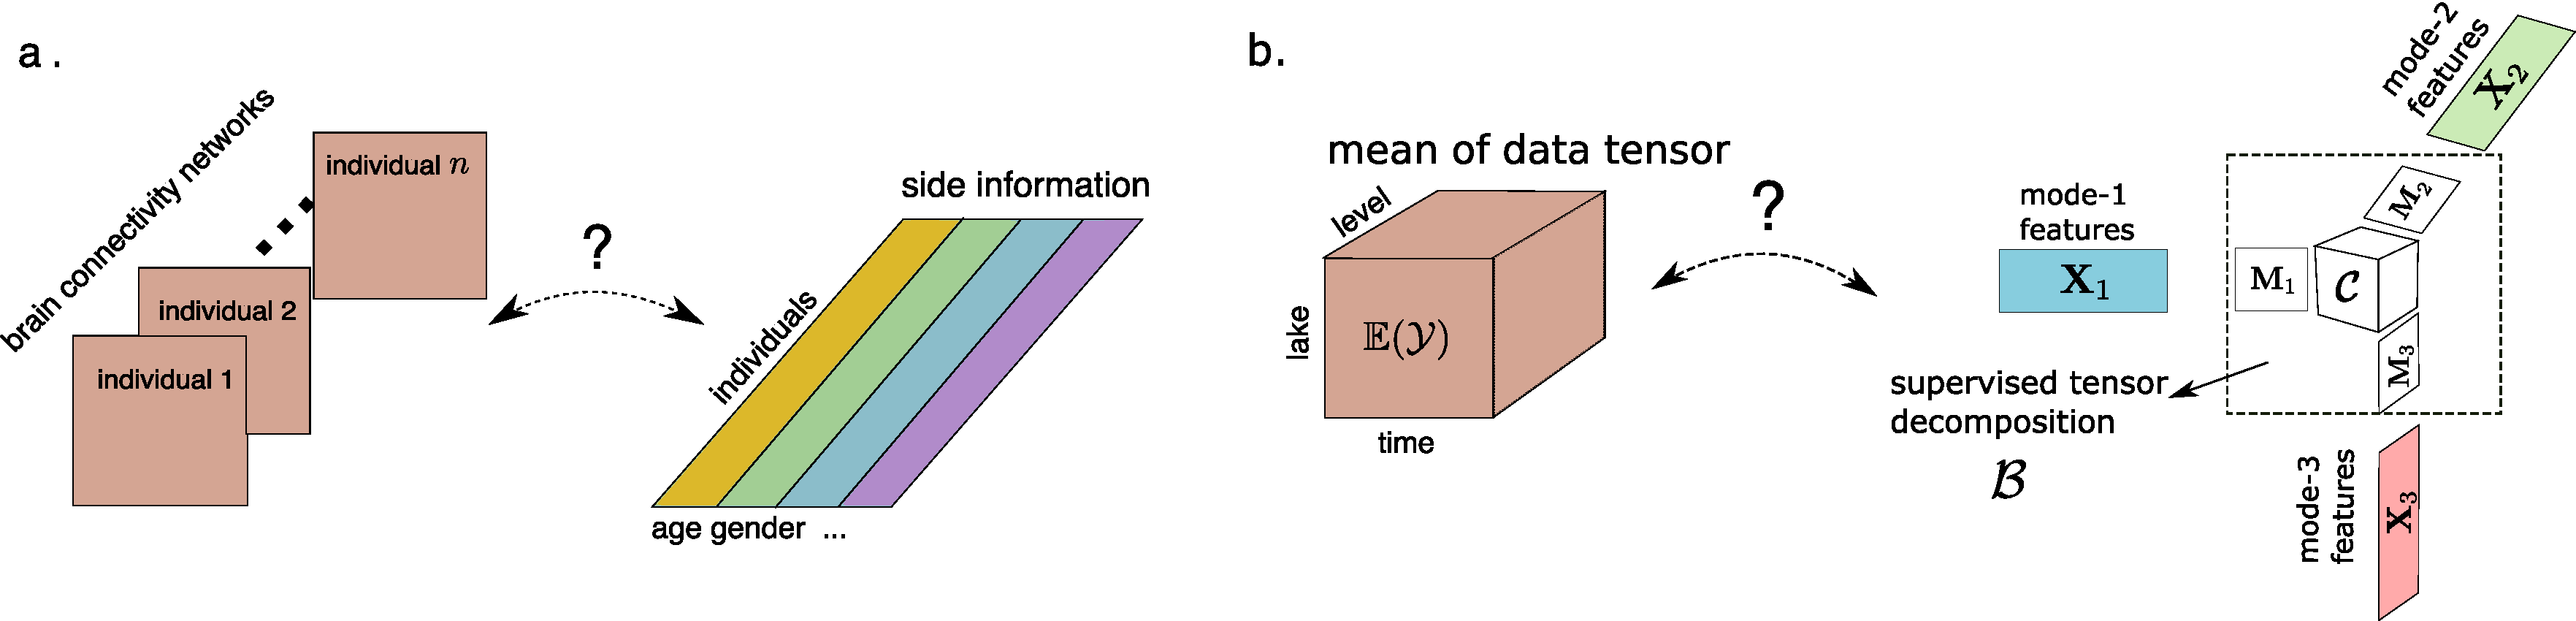
\includegraphics[width=16cm]{demo.pdf}
\end{center}
\caption{Examples of supervised tensor decomposition with interactive side information. (a) Network population model. (b) Spatial-temporal growth model as an example of supervised decomposition of an order-3 tensor $\tY$, where feature matrices $\mX_k$ are available on each of the three modes.}\label{fig:intro1}
\end{figure*}

\subsubsection{Proposed Framework for Supervised Tensor Learning} 
The proposed project focuses on developing a general model for decomposing a data tensor with exponential family entries and interactive side information. We will formulate the learning task as a structured regression problem, with tensor observation serving as the response, and the multiple side information as interactive features. Figure~\ref{fig:intro1}b illustrates our model in the special case of order-3 tensors. A low-rank structure is imposed to the conditional mean tensor, where unlike classical decomposition, the tensor factors $\mX_k\mM_k\in\mathbb{R}^{d_k\times r_k}$ belong to the space spanned by features $\mX_k\in\mathbb{R}^{d_k\times p_k}$ for $k=1,2,3$. The unknown matrices $\mM_k\in\mathbb{R}^{p_k\times r_k}$ (referred to as ``dimension reduction matrices'') link the conditional mean to the feature spaces, thereby allowing the identification of variations in the tensor data attributable to the side information. The tensor approach boosts the prediction performance by incorporating interactions across multiple modes. 


Our proposal blends the modeling power of generalized linear model (GLM) and the exploratory capability of tensor dimension reduction in order to take the best out of both worlds. We propose to leverage GLM to allow heteroscedacity in the non-Gaussian data. This flexibility is important in practice. Furthermore, our low-rank model on the possibly non-linearly transformed conditional mean tensor effectively mitigates the curse of high dimensionality. In classical GLM, the sample size and feature dimension are well defined; however, in the tensor data analysis, we observe only one realization of an order-$K$ tensor and up to $K$ interactive feature matrices. Both the number of tensor entries and feature dimension grow exponentially in $K$. Dimension reduction is therefore crucial for prediction and interpretability. We will establish the computational performance of our estimator, and we will quantify the gain in prediction in applications. 

\subsubsection{Three Examples}
We give three different examples to highlight the applicability of our supervised tensor learning methods.\\

\begin{example}[Spatio-temporal growth model]
The growth curve model~\cite{gabriel1998generalised,srivastava2008models} was originally proposed as an example of bilinear model for matrix data, and we adopt its higher-order extension here. Let $\tY=\entry{y_{ijk}}\in\mathbb{R}^{d \times m\times n}$ denote the pH measurements of $d$ lakes at $m$ levels of depth and for $n$ time points. Suppose the sampled lakes belong to $q$ types, with $p$ lakes in each type. Let $\{\ell_j\}_{j\in[m]}$ denote the sampled depth levels and $\{t_k\}_{k\in[n]}$ the time points. Assume that the expected pH trend in depth is a polynomial of order at most $r$ and that the expected trend in time is a polynomial of order $s$. Then, the conditional mean model for the spatio-temporal growth model can be represented as
\begin{equation}\label{eq:time}
\mathbb{E}(\tY|\mX_1,\mX_2,\mX_3)=\tC\times\{\mX_1\mM_1,\ \mX_2\mM_2,\ \mX_3\mM_3\},
\end{equation}
where $\mX_1=\text{blockdiag}\{\mathbf{1}_p,\ldots,\mathbf{1}_p\}\in \{0,1\}^{d\times q}$ is the design matrix for lake types, and
\[
\mX_2=
\begin{pmatrix}
1 & \ell_1&\cdots &\ell^{r}_1\\
1 & \ell_2&\cdots &\ell^{r}_2\\
\vdots &\vdots&\ddots&\vdots\\
1&\ell_{m}&\cdots&\ell^{r}_{m}
\end{pmatrix},\quad
\mX_3=
\begin{pmatrix}
1 & t_1&\cdots &t^{s}_1\\
1 & t_2&\cdots &t^{s}_2\\
\vdots &\vdots&\ddots&\vdots\\
1&t_{n}&\cdots&t^{s}_{n}
\end{pmatrix}
\]
are the design matrices for spatial and temporal effects, respectively, $\tC\in\mathbb{R}^{r_1\times r_2\times r_3}$ is the unknown core tensor, and $\mM_k$ are unknown dimension reduction matrices along each mode. The factors $\mX_k\mM_k$ are sufficient features for the mean model~\eqref{eq:time}. The spatial-temporal model is a special case of our supervised tensor decomposition model, with features available on each of the three modes.\\
\end{example}


\begin{example}[Network population model]\label{example:brain}
Network response model~\cite{rabusseau2016low, zhang2018network} is recently developed for neuroimanig analysis. The goal is to study the relationship between brain network connectivity pattern and features of individuals. Suppose we have a sample of $n$ observations, $\{(\mY_i, \mx_i)\colon i=1,\ldots,n\}$, where for each individual $i\in[n]$, $\mY_i\in\{0,1\}^{d\times d}$ is the symmetric adjacency matrix whose entries indicate presences/absences of connectivities between $d$ brain nodes, and $\mx_i\in\mathbb{R}^p$ is the individual's feature such as age, gender, cognition score, etc. The network-response model  has the conditional mean
\begin{equation}\label{eq:network}
\textup{logit}(\mathbb{E}(\mY_i|\mx_i))=\tB\times_3\mx_i, \quad \text{for }i=1,\ldots,n,
\end{equation}
where $\tB\in \mathbb{R}^{d\times d\times p}$ is a rank-$(r_1,r_1,r_2)$ coefficient tensor that is symmetric in the first two modes.  

The model~\eqref{eq:network} is a special case of our supervised tensor decomposition, with feature matrix on the last mode of the tensor. Specifically, we stack the network observations $\{\mY_i\}$ together and obtain an order-3 response tensor $\tY\in\{0,1\}^{d\times d\times n}$. Define a feature matrix $\mX=[\mx_1,\ldots,\mx_n]^T\in\mathbb{R}^{n\times p}$. Then, the model~\eqref{eq:network} has the equivalent representation of supervised tensor decomposition,
\[
\textup{logit}(\mathbb{E}(\tY|\mX))=\tC\times\{\mM,\ \mM,\ \mX\mM'\},
\]
where $\tC\in\mathbb{R}^{r_1\times r_1\times r_2}$ is the core tensor, $\mM\in\mathbb{R}^{d\times r}$ is the dimension reduction matrix at the first two modes, and $\mM'\in\mathbb{R}^{p\times r_2}$ is for the last mode.\\
 \end{example}
 
 \begin{example}[Dyadic data with node attributes] Dyadic dataset consists of measurements on pairs of objects or under a pair of conditions. Common examples include graphs and networks. Let $\tG=(V,E)$ denote a graph, where $V=[d]$ is the node set of the graph, and $E\subset V\times V$ is the edge set. Suppose that we also observe feature vector $\mx_i\in\mathbb{R}^p$ associated to each $i\in V$. A probabilistic model on the graph $\tG=(V,E)$ can be described by the following matrix regression. The edge connects the two vertices $i$ and $j$ independently of other pairs, and the probability of connection is modeled as
\begin{equation}\label{eq:edge}
 \textup{logit}\left(\mathbb{P}\left((i,j)\in E\right)\right)=\mx^T_i\mB\mx_j=\langle \mB,\ \mx^T_i\mx_j\rangle,
 \end{equation}
 where $\mB\in\mathbb{R}^{p\times p}$ is a symmetric rank-$r$ matrix. The low-rankness in $\mB$ has demonstrated its success in modeling transitivity, balance, and communities in the networks~\cite{hoff2005bilinear}. Our supervised tensor decompostion also incorporates the graph model as a special case. Let $\tY=\entry{y_{ij}}$ be a binary matrix where $y_{ij}=\mathds{1}_{(i,j)\in E}$. Define $\mX=[\mx_1,\ldots,\mx_n]^T\in\mathbb{R}^{n\times p}$. Then, the graph model~\eqref{eq:edge} can be expressed as
 \[
 \textup{logit}(\mathbb{E}(\mY|\mX))=\mC\times\{\mX\mM,\ \mX\mM\}, 
  \]
  where $\mC\in\mathbb{R}^{r\times r}$ and $\mM\in\mathbb{R}^{p\times r}$ are based on the singular value decomposition of $\mB=\mM\mC\mM^T$. 
  \end{example}
  

\subsubsection{Significance and Challenges}
In the above three examples and many other studies, researchers are interested in uncovering the variation in the data tensor that can be explained by features. The coefficient tensor $\tB$ in model~\eqref{eq:network} serves this goal by collecting the feature effects. To encourage the sharing among effects, decomposition in Figure~\ref{fig:intro1}b assumes that the feature effects $\tB$ lie in a low-dimensional parameter space. The low-rank assumption is plausible in many scientific applications. In the Example~\ref{example:brain} of brain imaging analysis, for instance, it is often believed that the brain nodes can be partitioned into several regions, and the person's attributes affect the connectivity in a similar way within a region. 

Learning tensors with interactive side information is challenging because of the extremely high dimensionality in both the tensor space and feature space. The PI's previous extensive experience on tensor related work has shown that tensors sought in applications often possess special structures, such as (nearly) low-rankness, sparsity, non-negativity, or orthogonal decomposability. We will leverage the formalisms of \emph{intrinsic dimension} to develop efficient statistical methods for analyzing these high-dimensional datasets. We will further develop adaptive, semi-supervised methods that incorporate practical constraints in industrial applications, such as incomplete observation with missing labels, corrupted distributions, and computation with time and memory constraints. 

\mybox[gray!20]{{\bf Impact and Significance:} 
\begin{itemize}[leftmargin=*]
\item Develop efficient prediction tools for tensor classification, tensor regression, and deep tensor neural network in the presence of domain constraints.
\item Build data-driven prototypes that integrate machine learning into the data-to-decision process. 
\item Improve efficiency in scientific discovery using powerful multi-modal brain imaging analyses. 
\end{itemize}
}


\section{Borader Impacts}
The educational components of this proposal are targeted at several different populations of students: PhD students, undergraduate students, visiting international students, AP statistics students underrepresented students at Mid-west area of United States. The project will support the development of the PI, a young faculty, to create an interdisciplinary working group of researchers.


\subsection{Diversity and My Past Experience}
I am one of the few female faculty members in my home department. As a young faculty, I have been striving to encourage more under-represented students into the field of machine learning. I am currently starting my third year in the tenure track, and I have successfully mentored a number of female undergraduate students -- two of which are embarking their PhD studies at top US universities this fall. Female students are traditionally underrepresented in my filed, and I have been striving to retain more women in the academic research. For that reason, I have sponsored my students to present their research in top-notch machine learning conferences including Conference on Neural Information Processing Systems (NeurIPS) and International Conference of Machine Learning (ICML). My experience of recruiting under-represented students has attracted social media coverage, and I was recently featured in the article ``Women in STEM: 5 Thoughtful Ways to Recruit and Retain Them'' by Course Hero Faculty Club . With the support of Sony research grant, I will be excited to further extend this effort to a larger student body. 


In addition, I have been devoted myself to general higher education. I am one of the core members in Madison Teaching and Learning Excellence program. I plan to create an undergraduate course on introduction to data sciences. This course will expose undergraduate students to a wide range of modern exploratory analytic tools for massive high-dimensional data, and will be closely tied with data-intensive scientific domains. Machine learning, as a discipline, is concerned with transforming “data” into “information”. However data are not just numbers, they are numbers with social, economical, and cultural contexts. The personnel constitution in our education environment is becoming increasingly diverse, reflecting the variety witnessed in our broader society. Diversity can be measured across many dimensions – gender, ethnicity, origin, age, etc. However, diversity is not limited to these visible physical differences; it also consists of difference in each student’s personality (introvert vs. extravert), learning skills (listening, speaking, reading, or writing skills), emotional development, and every aspect that distinguishes one individual from another. I believe that every student is unique in their own way, and I have been striving to create an open, inclusive education environment that prepares students to become better professionals in the larger, diverse society.

\subsection{Deliverables and Milestones}
The project will create deliverables in three aspects: {\bf research}, {\bf education}, and {\bf social good}. I plan to devote one year for each of the aforementioned research problems. My current group consists of three PhD students and two undergraduates, of which three are females (me included) and three are males. I have actively contributed to several multi-institutional consortiums, in collaboration with researchers in United States, Europe, and Asia. The Sony grant will support me to further create a diverse working group. Regarding teaching, I will create a new course on \emph{data science} in both traditional and online formats. The new course will introduce students to the real word challenges in implementing statistical machine learning approaches to decision making. I will also organize a series of workshops on the scientific applications of tensor data analysis, with the aim to encourage interdisciplinary collaborations. Figure~\ref{fig:proposal} summarizes the planned milestones for my proposal. 


\begin{figure}[!h]
\begin{center}
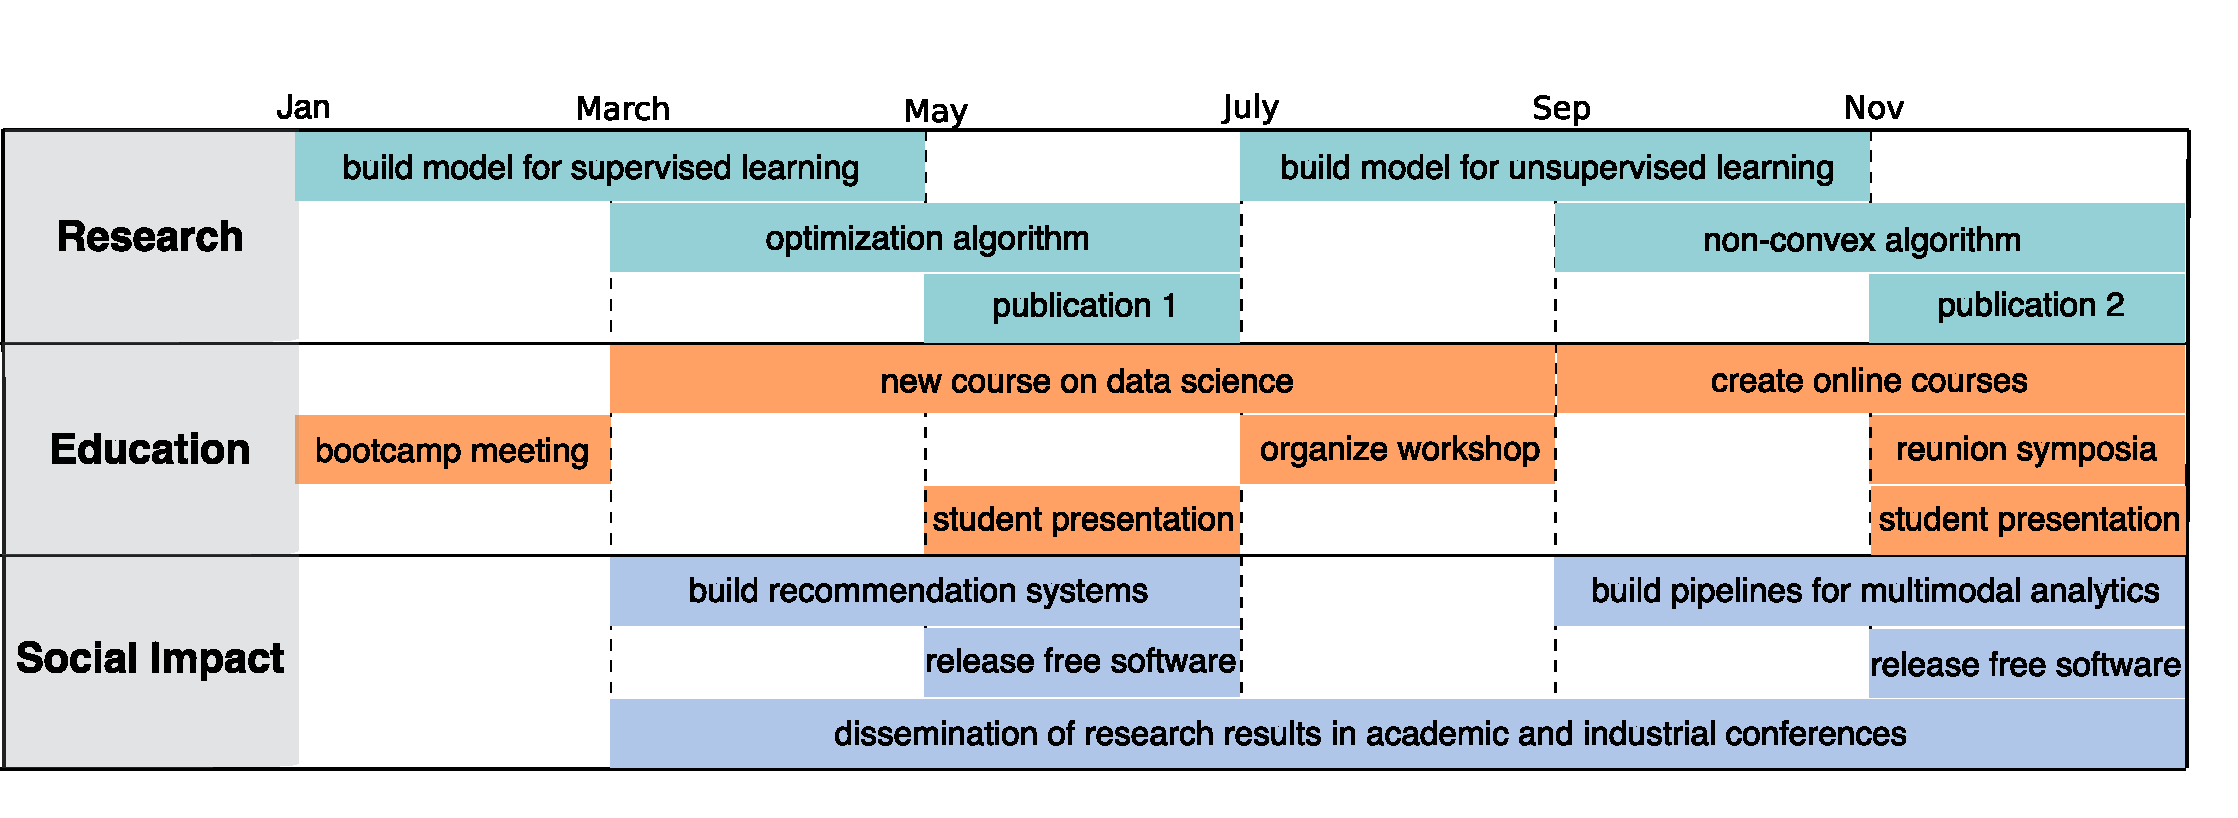
\includegraphics[width=.98\textwidth]{milestone.pdf}
\vspace{-.4cm}
\caption{Planned deliverables and milestones for my proposal.}\label{fig:proposal}
\end{center}
\vspace{-.4cm}
\end{figure}

\subsection{Other Outreaches}
I have a unique combination of training backgrounds in statistics, computer science, and scientific research. My established collaborations on cutting-edge scientific problems has motivated the methodological ideas presented in this proposal. Ongoing collaborations include research groups at University of Pennsylvania, University of Chicago, University of California-Berkeley, and data science group at Chan Zuckerberg Biohub. The resulting solutions are expected to have a direct impact on a broad range of scientific and engineering fields. Open-source software will be released, as the fruit of the research, that facilitates academia, industry, and society to analyze complicated large-scale data. 

\bibliography{tensor_wang}
\bibliographystyle{plain}


\end{document}